\documentclass{article} % JASA requires 12 pt font for manuscripts
%\usepackage{JASA_manu}        % For JASA manuscript formatting

%\usepackage{endfloat} % just for while I am writing

% for citations
\usepackage[authoryear]{natbib} % natbib required for JASA
\usepackage[colorlinks=true, citecolor=blue, linkcolor=blue]{hyperref}

% for the fancy tables with the icons
%\usepackage[margin=1.0in]{geometry}% http://ctan.org/pkg/margin
\usepackage{booktabs}% http://ctan.org/pkg/booktabs
\usepackage{array}% http://ctan.org/pkg/array
\newcolumntype{M}{>{\centering\arraybackslash}m{\dimexpr.05\linewidth-2\tabcolsep}}



%\definecolor{Blue}{rgb}{0,0,0.5}
\newcommand{\hh}[1]{{\color{orange} #1}}
\newcommand{\al}[1]{{\color{red} #1}}

% fonts
%\usepackage{kpfonts}

% for figures
\usepackage{graphicx}
\DeclareGraphicsExtensions{.eps, .pdf}
\graphicspath{{figures/}}

% help with editing and coauthoring
\usepackage{todonotes}
\newcommand{\alnote}[1]{\todo[inline,color=green!40]{#1}}

% title formatting
\usepackage[compact,small]{titlesec}

% page formatting
\usepackage[margin = 1in]{geometry}
\usepackage[parfill]{parskip}

% line spacing
\usepackage{setspace}
\doublespace

% For math typsetting
\usepackage{bm}
\usepackage{amstext}
\usepackage{amssymb}
\usepackage{amsmath}
\usepackage{amsfonts}
\usepackage{multirow}

% A few commands to make typing less tedious
\newcommand{\inv}{\ensuremath{^{-1}}}
\newcommand{\ginv}{\ensuremath{^{-}}}
\newcommand{\trans}{\ensuremath{^\prime}}
\newcommand{\E}{\ensuremath{\mathrm{E}}}
\newcommand{\var}{\ensuremath{\mathrm{Var}}}
\newcommand{\cov}{\ensuremath{\mathrm{Cov}}}


\title{Title: Something Creative about Q-Q Plots}

\author{Adam Loy, Lendie Follett, Heike Hofmann}

\begin{document}
\maketitle

\alnote{From my dissertation}

The lineup protocol also allows for an assessment of the power of a lineup \citep{mahbub:2013}. 
%as the probability that in $N$ independent evaluations observers 
In $N$ independent evaluations, the probability that observers
choose the true plot more than $x_\alpha$ times is
\begin{equation}\label{eqn:power}
\widehat{\text{Power}} = \text{Power}_{N} = 1 - F_{X} (x_{\alpha}),
\end{equation}
where $F_X$ is the distribution of $X$ and $x_\alpha$ is the critical value for a given significance level of $\alpha$, i.e. $P(X >  x_{\alpha}) \le \alpha$. $X$ is composed of the sum of $N$ observers' (binary) decisions $X_i \sim B_{1, p_i}$, where  $p_i$ is the probability that individual $i$ chooses the data plot. This probability  depends both on the strength of the signal in the data plot and an individual's visual ability.
Assessing this ability requires that each individual evaluates multiple lineups. If that is not possible, we have to assume that all participants share the same ability, and the power calculation in Equation~\ref{eqn:power} simplifies to $1 - B_{N, \hat{p}}(x_\alpha)$, where $\widehat{p}$ is an estimate for the probability of choosing the data plot for a specific lineup. Similar to classical inference, we can make use of power to assess sensitivity of tests. This allows us to make decisions about designs for particular tasks by evaluating lineups displaying \hh{  the same data in different types of displays} \citep{Hofmann:2012ts}. 

%------------------------------------------------------------------------------------
\subsubsection{Investigating Q-Q plots visually}\label{sec:qqplot}
%------------------------------------------------------------------------------------

To further \al{develop} the assessment of normality using lineups, we conducted a study comparing three different versions of the Q-Q plot.
%We are testing three different versions of a Q-Q plot, 
Examples of the three versions are displayed in Figure~\ref{qqplots} and include (from left to right): a \emph{control} Q-Q plot, a \emph{standard} Q-Q plot with an added grey band representing a 95\% pointwise confidence region based on the estimated standard error of the order statistics for an independent sample from the theoretical distribution,
 and a \emph{rotated} (i.e., detrended) Q-Q plot. All Q-Q plots in Figure~\ref{qqplots} are constructed from the same data. To explore the results of this study we must first define some additional notation.

\begin{figure}
%<<qqplots, fig.width=2.75, fig.height=2.75, out.width='0.3\\textwidth', echo=FALSE, include=FALSE>>=
%dframe <- read.csv("data/data-1-1-1-20-2-14-5.csv")
%library(ggplot2)
%dframe$.sample <- "Control"
%ctrl_lineup(subset(dframe, .sample_outer==5))
%dframe$.sample <- "Standard"
%std_lineup(subset(dframe, .sample_outer==5))
%dframe$.sample <- "Rotated"
%rot_lineup(subset(dframe, .sample_outer==5))
%@
\centering
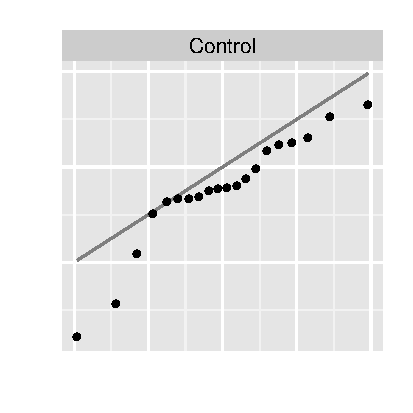
\includegraphics[width=0.3\textwidth]{qqplots1}
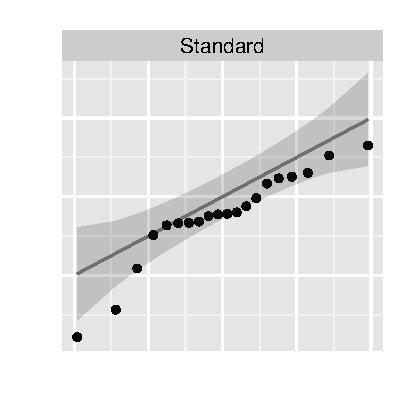
\includegraphics[width=0.3\textwidth]{qqplots2}
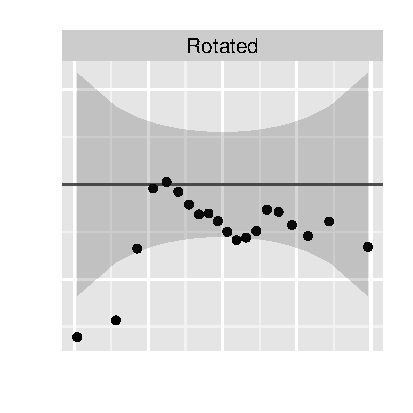
\includegraphics[width=0.3\textwidth]{qqplots3}
\caption{ \label{qqplots} Three versions of Q-Q plots: control, standard, and rotated.}
\end{figure}


Let $X_i \sim B_{1, \pi_i}, 1 \le i \le n$, where $X_i$ is the binary decision on the $i$th evaluation and $\pi_i$ is the probability with which the observer chooses the data plot. This probability is influenced by a number of factors:

\begin{center}
\begin{tabular}{lp{5in}}
$\tau$ & the design used in the lineup (Control, Standard, Rotated), \\
&  the specific parameters under which the data for the lineup were created: \\
&  $\delta$ \ \ \ degrees of freedom (2, 5, 10) {of the $t$ distribution} and \\
&  $\nu$  \ \ \ sample size (10, 20, 50, 75), \\
$d$ &  the level of difficulty based on the actual sample, and \\
$u$ & the users' subjective abilities.
 \end{tabular}
\end{center}
%
The above factors result in 12 different parameter settings. For each setting we created two samples, along with two null data sets each, yielding 48 different lineups. 
Using  Amazon MTurk \citep{amazon}, 417 participants were each asked to evaluate ten different lineups. 
We model the probability of selecting the data plot from the lineup, $\pi$, with the help of model $M_1$:
\[
g(\pi_i) = \mu + \tau_{j(i)} +\delta_{k(i)}+ \nu_{s(i)} + u_{u(i)} + d_{d(i)}
\]
where $g$ is the logit link function, and $j(.), k(.), s(.), u(.)$, and $d(.)$ are all indexing functions that relate evaluation $i$ to the corresponding levels in the factor variables, to the observer, or a particular data sample. More specifically, $j(i) \in \{$Control, Standard, Rotated$\}$; $k(i) \in \{2,5,10\}$; $s(i) \in \{20, 30, 50, 75\}$; $u(i)$ maps to the participant's id of the $i$th evaluation and $d(i)$ identifies the particular data sample used for it. 

Both user ability, $u$, and sample difficulty, $d$, are modeled as independent, normally distributed  random effects, i.e. $u_{u(i)} \sim N(0, \sigma_u^2)$, $d_{d(i)} \sim N(0,\sigma_d^2)$ with cov$(u, d) = 0$.



%\begin{center}
%\begin{tabular}{lp{5.5in}}
%$\mu$ & overall mean\\
%$\tau_{j(i)}$ & is the effect of design $j$, $j \in \{ \text{Control, Standard, Rotated} \}$, and $j(i)$ is the design used in evaluation $i$, $1 \le i \le n$.  \\
%$\delta_{k(i)}$ & is the effect of $k$ degrees of freedom , $k \in \{ 2, 5, 10 \}$, and $k(i)$ is the degree of freedom used to generate the lineup  in evaluation $i$, $1 \le i \le n$.  \\
%$\nu_{\ell(i)}$ & is the effect of sample size $\ell$, $\ell \in \{ 20, 30, 50, 75 \}$, and $\ell(i)$ is the sample size used to generate the lineup  in evaluation $i$, $1 \le i \le n$.  \\
%$u_{u(i)}$ & user ability, $u_{u(i)} \sim N(0,1)$ i.i.d \\
%$d_{\ell(i)}$ & data difficulty, $d_{\ell(i)} \sim N(0,1)$ i.i.d 
%\end{tabular}
%\end{center}

% latex table generated in R 3.0.1 by xtable 1.7-1 package
% Sun May 26 13:36:30 2013
% xtable(summary(m0)@coefs, digits=c(0,2,3,2,4))
\begin{table}[ht]
\centering
\caption{\label{tab:model} Coefficients and significances corresponding to  model $M_1$. The type of design is important for the power of a lineup. Rotated Q-Q plots lose a significant amount of power compared to both the regular and the standard version of Q-Q plots. }
\begin{tabular}{rrrrrl}
  \hline
 &\bf Estimate &\bf Std. Error &\bf z value &\bf Pr($>$$|$z$|$) & \\ 
  \hline
Intercept & -5.04 & 0.769 & -6.55 & 0.0000 & *** \\ [3pt]
\multicolumn{3}{l}{\bf design} \\
   Control & 0.00 & ----- & ----- & ----- \\ 
   Rotated & -0.38 & 0.128 & -2.97 & 0.0030 & **\\ 
   Standard & 0.11 & 0.127 & 0.88 & 0.3782 \\ [3pt]
%  locationOuter & 0.19 & 0.106 & 1.83 & 0.0677 \\ 
%  clickSingle & -0.09 & 0.104 & -0.89 & 0.3747 \\ 
\multicolumn{4}{l}{\bf degrees of freedom} \\
  2 & 6.32 & 0.743 & 8.50 & 0.0000 & ***\\ 
  5 & 2.43 & 0.726 & 3.34 & 0.0008 & ***\\ 
  10 & 0.00 & ----- & ----- & ----- \\ [3pt]
\multicolumn{3}{l}{\bf sample size} \\
  20 & 0.00 & ----- & ----- & ----- \\ 
  30 & 1.09 & 0.844 & 1.29 & 0.1970 \\ 
  50  & 2.98 & 0.844 & 3.54 & 0.0004 & ***\\ 
  75 & 2.31 & 0.845 & 2.73 & 0.0063  & **\\ 
   \hline
\multicolumn{5}{l}{Signif. codes:  0 �***� 0.001 �**� 0.01 �*� 0.05 �.� 0.1 � � 1}
\end{tabular}
\end{table}

The estimated model coefficients for model $M_1$ are shown in Table~\ref{tab:model}. 
\hh{Estimates of the variance components are $\widehat{\sigma}_u = 0.71$, $\widehat{\sigma}_d=1.95$, and $\widehat{\sigma} = 0.29$. Variances of user ability and data difficulty are large relative to residual variance, indicating that both random effects are necessary.}
%
As expected, the task of identifying non-normality is easier with increased sample size and more pronounced deviations from normality, as is the case with lower degrees of freedom. The  design of the Q-Q plot is of huge importance for the probability of choosing the data plot. Interestingly, the rotated version of the Q-Q plot is significantly less suitable for the task of assessing normality compared to the control. Additionally, adding confidence bands helps with evaluation, but not significantly. 

Note that none of the data plots in the lineups were actually created using data from a normal distribution. This should lead to rejection of the null hypothesis in every single instance. This is not quite true, as can be seen in Table~\ref{tab:reject}, but what also becomes evident is the high power  of visual inference. Based on lineups we are able to reject non-normality much more often than with any of the classical tests.

% latex table generated in R 3.0.1 by xtable 1.7-1 package
% Mon May 27 20:57:50 2013
\begin{table}[ht]
\centering
\caption{\label{tab:reject} 
Out of the 48 non-normal samples, 24 get rejected at the 5\% significance level based on evaluation by observers. None of the classical tests come close to that rejection rate. From left to right, we see the number of rejections from visual inference as well as the Anderson-Darling, Shapiro-Wilk, Cram\'er-von Mises and Kolmogorov-Smirnov tests for normality.}
\begin{tabular}{rrrrrr}
  \hline
Result & Visual & AD & SW & CVM & KS \\ 
  \hline
  reject & 24 & 10 & 16 &  8 & 10 \\ 
  not reject & 24 & 38 & 32 & 40 & 38 \\ 
   \hline
\end{tabular}
\end{table}


\end{document}